\documentclass{article}
\usepackage{graphicx}

\title{Hardware Assignment Report}
\author{Name: ANURAG\\Roll Number: BT22BTECH11002}
\date{}

\begin{document}
\maketitle

\section{Aim}
In this assignment, we have made a Random number generator using shift registers.

\section{Procedure}
\begin{enumerate}
  \item We connected the 555 timer circuit.
  \item Then we connected the Clock output of the 555 timer circuit to the clock signal of D-Flip flops.
  \item Now we make the circuit for shift registers using 4 D-Flip flops (using two 7474 IC's).
  \item Then we connected XOR gate (7486 IC).
  \item We connected the decoder (7447 IC) and connected its A, B, C, D with Q0, Q1, Q2, Q3 respectively.
  \item Then we connected the seven-segmented display and connected it with the decoder (7447 IC).
  \item We connected all the independent parts with each other and then connected the power source.
\end{enumerate}

\section{Conclusion}
The output was changing digits on the seven-segment display.

\section{Circuit Image}
\begin{figure}[ht]
  \centering
  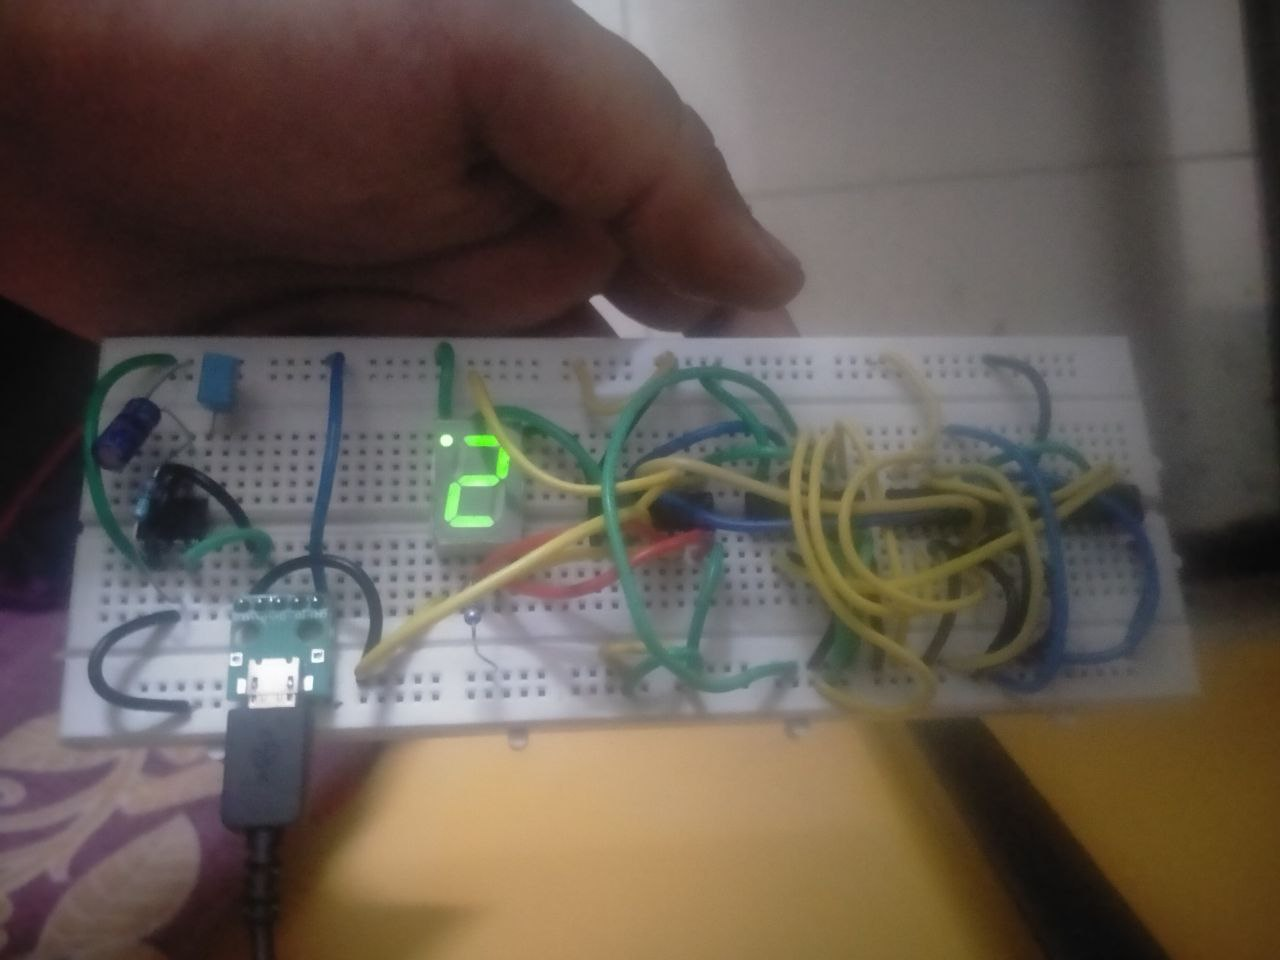
\includegraphics[width=\textwidth]{circuit.jpg}
  \caption{circuit image }
  \label{fig:circuit}
\end{figure}

\end{document}
